\documentclass[sokoban_generation_thesis.tex]{subfiles}
Metoda SYM \cite{heur_sim} opiera swoje działanie na~symulowaniu zmodyfikowanej rozgrywki \textit{Sokoban}. Iteracyjnie wykonując pewne akcje i~przechodząc po~początkowo pustej planszy, agent wyznacza wolne pola.

\subsection{Opis metody}
Metoda SYM rozpoczyna pracę, losując początkowe ustawienia pudeł na~planszy. Następnie agent wykonuje założoną liczbę razy dwa rodzaje rozgrywek: najpierw rozgrywki typu \textit{forward}, a~następnie -- \textit{backward}, by~potem uporządkować generowaną planszę.

W rozgrywce \textit{forward}, agent wybiera w~określony sposób pudło i~kierunek jego przepychania, by~dokonać przepchnięcia. Jeśli przepchnięcie jest możliwe, to~pudło zmienia swoją pozycję, a~pola przez które przeszedł agent, stają się pustymi polami. Przykładowo, jeśli dla planszy na~rys.~\ref{rys:board_sym_pre} gracz wybierze wyższe pudło i~dół jako kierunek przepychania, to~jego akcja spowoduje że~plansza przybierze układ jak na~rys.~\ref{rys:board_sym_post}.

\begin{figure}[h]
	\centering
	\begin{subfigure}[b]{0.35\textwidth}
		\centering
		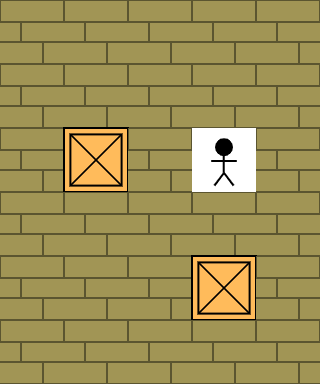
\includegraphics[width=0.5\textwidth]{board_sym_pre}
		\caption{Plansza przed wykonaniem akcji}
		\label{rys:board_sym_pre}
	\end{subfigure}
	\hspace{0.1\textwidth}
	\begin{subfigure}[b]{0.35\textwidth}
		\centering
		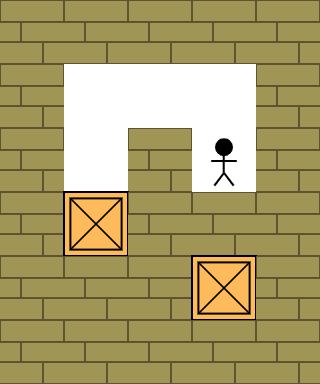
\includegraphics[width=0.5\textwidth]{board_sym_post}
		\caption{Plansza po~wykonaniu akcji}
		\label{rys:board_sym_post}
	\end{subfigure}
	\hspace{0.15\textwidth}
	\begin{subfigure}[b]{0.5\textwidth}
		\centering
		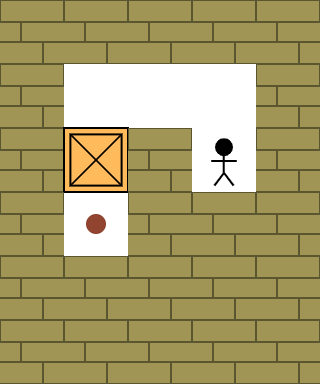
\includegraphics[width=0.35\textwidth]{board_sym_transform}
		\caption{Plansza po~zakończeniu rozgrywki}
		\label{rys:board_sym_transform}
	\end{subfigure}
	\caption{Działanie akcji w~rozgrywce \textit{forward}}
\end{figure}

Po zakończeniu rozgrywki \textit{forward}, pudła zamieniane są~w~pola docelowe, a~startowe pozycje pudeł stają się faktycznymi pudłami. Ponadto, nieprzepchnięte pudła zamieniane są~w~ściany. Kontynuując analizę przypadku, jeśli rozgrywka \textit{forward} zostanie zakończona z~planszą jak na~rys.~\ref{rys:board_sym_post}, to~w~wyniku transformacji otrzyma się planszę przedstawioną na~rys.~\ref{rys:board_sym_transform} i~agent przejdzie do~przeprowadzenia rozgrywki \textit{backward}, w~celu dodatkowego skomplikowania planszy.

W rozgrywce \textit{backward}, agent wybiera w~określony sposób pudło i~kierunek jego przeciągania. Akcja przeciągnięcia jest akcją niedostępną w~normalnej rozgrywce \textit{Sokoban} i~działa odwrotnie do~akcji przepychania. W~wyniku tej akcji, jeśli przeciągnięcie jest możliwe, to~pudło oraz gracz aktualizują swoje pozycje. Przykładowo, jeśli dla planszy na~rys.~\ref{rys:board_sym_pre_back} gracz wybierze jedyne dostępne pudło i~górę jako kierunek przeciągania, to~jego akcja spowoduje że~plansza przybierze układ jak na~rys.~\ref{rys:board_sym_post_back}. 

\begin{figure}[h]
	\centering
	\begin{subfigure}[b]{0.35\textwidth}
		\centering
		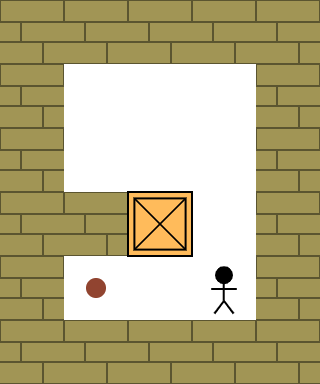
\includegraphics[width=0.5\textwidth]{board_sym_pre_back}
		\caption{Plansza przed wykonaniem akcji}
		\label{rys:board_sym_pre_back}
	\end{subfigure}
	\hspace{0.15\textwidth}
	\begin{subfigure}[b]{0.35\textwidth}
		\centering
		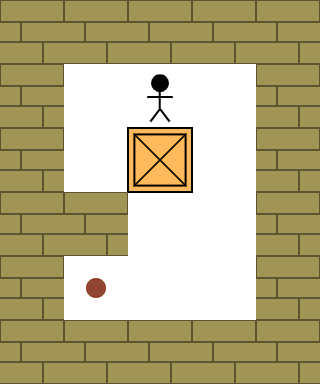
\includegraphics[width=0.5\textwidth]{board_sym_post_back}
		\caption{Plansza po~wykonaniu akcji}
		\label{rys:board_sym_post_back}
	\end{subfigure}
	\caption{Działanie akcji w~rozgrywce \textit{backward}}
\end{figure}

\subsection{Strategie} \label{sub:sym_strategie}

\begin{table}[h!]
	\smallskip
	\centering
	\begin{tabular}{|l|l|l|l|}
		\hline
		\textbf{Wybór pudła} & \textbf{Kierunek} & \textbf{Kierunek} & \textbf{Wybór ścieżki} \\ 
		& \textbf{przepychania} & \textbf{przeciągania} &  \\\hline
		\textit{Random} & \textit{Random} & \textit{Random} & \textit{Direct}\\
		\textit{Least Pushed} & \textit{Farthest} & \textit{Farthest} & \textit{Closest Active Tile}\\
		\textit{In Order} & \textit{Most Obstacles} & \textit{Most Obstacles}& \\
		& & \textit{Most Access}& \\
		\hline
	\end{tabular}
	\caption{Strategie decyzyjne metody SYM}
	\label{tab:sym_strategies}
\end{table}

W procesie generowania planszy metody SYM, agent podejmuje decyzje o~przepychaniu i~przeciąganiu pudeł oraz o~sposobie wyboru ścieżek. Wybory dokonywane są~zgodnie z~ustalonymi wcześniej strategiami, będącymi hiperparametrami metody. Wszystkie strategie, które zostały zaprezentowane w~pracy wprowadzającej metodę SYM, zostały wymienione w~tab.~\ref{tab:sym_strategies}.

Strategie \textit{Random} dokonują wyborów w~sposób losowy. Strategia \textit{Least Pushed} wybiera te~pudła, które w~momencie podejmowania decyzji zostały przepchnięte najmniejszą liczbę razy, a~\textit{In Order} -- wybiera pudła po~kolei, niezależnie od~liczby przepchnięć.~\textit{Farthest} maksymalizuje odległość od~pudła do~jego pola docelowego.~\textit{Most Obstacles} wybiera kierunek tak, by~wynikowa pozycja pudła sąsiadowała z~jak największą liczbą ścian i~innych pudeł.~\textit{Most Access} ma~zapewnić agentowi jak najwięcej dostępnych kierunków po~wykonaniu akcji przeciągania. Strategia wyboru ścieżek \textit{Closest Active Tile} stara się wykorzystać jak najwięcej już odwiedzonych pól, zachowując w~ten sposób więcej ścian niż odpowiadająca jej strategia \textit{Direct}, która wybiera najkrótsze możliwe ścieżki.


